\documentclass[10pt, xcolor=table]{beamer}
%
% Packages
\usepackage[english]{babel} % Set language
\usepackage[T1]{fontenc}  % font Encoder for westeuropean languages
\usepackage[utf8]{inputenc} % Utf8 input encoder
\usepackage[autostyle=true,german=quotes]{csquotes} % quotation package
\usepackage[ddmmyyyy]{datetime} % for date and time formats
\usepackage[sorting=none,backend=biber]{biblatex}  % bibliography package
\usepackage{pgfpages} % print multiple pages per slide
\usepackage[font={footnotesize}]{caption} %caption package
\usepackage{xcolor} % color package
\usepackage{subfigure}
%\usepackage{ziffer} % set , as decimal and . as thousand seperator (needed for german)
%
%
% activate to show notes on second screen:
%\setbeameroption{show notes on second screen}
%
%
% Bibliography
\addbibresource{references.bib}
%
% Image Path
\graphicspath{{Images/}}
%
% Style
% Define style
\usetheme{Boadilla}
\useoutertheme{miniframes}
\useinnertheme{rectangles}

% Define colours
\definecolor{THblack}{HTML}{000000}
\definecolor{THRed}{RGB}{201,12,15}
\definecolor{THOrange}{RGB}{234,91,12}
\definecolor{THPurple}{RGB}{184,37,133}
\definecolor{BlueSaphirre}{HTML}{0B4F6C}
\definecolor{DartmouthGreen}{HTML}{306B34}

% define element colors
\setbeamercolor{palette primary}{bg=THPurple,fg=white}
\setbeamercolor{palette secondary}{bg=THRed,fg=white}
\setbeamercolor{palette tertiary}{bg=THOrange,fg=white}
\setbeamercolor{palette quaternary}{bg=THblack,fg=white}
\setbeamercolor{structure}{fg=THblack}
\setbeamercolor{title}{fg=THRed}
\setbeamercolor{frametitle}{fg=THOrange}
\setbeamercolor{mini frame}{fg=white, bg=THOrange}
\setbeamercolor{section in head/foot}{fg=white, bg=THOrange}
\setbeamercolor{structure}{fg=THblack}

% define Block colors
\setbeamercolor{block title}{bg=BlueSaphirre!50, fg=white}
\setbeamercolor{block body}{bg=BlueSaphirre!15}
\setbeamercolor{block title alerted}{bg=THRed!50, fg=white}
\setbeamercolor{block body alerted}{bg=THRed!15}
\setbeamercolor{block title example}{bg=DartmouthGreen!55, fg=white}
\setbeamercolor{block body example}{bg=DartmouthGreen!15}

% define element styles
\setbeamertemplate{headline}{}
\setbeamertemplate{section in toc shaded}[default][50]
\setbeamertemplate{section in toc}[square]
\setbeamertemplate{subsection in toc}[square]
\setbeamertemplate{itemize items}[square]
\setbeamertemplate{enumerate items}[square]
\setbeamertemplate{caption}[numbered]
\setbeamertemplate{blocks}[default]

% Show numbers instead of symbols in bibliography
\setbeamertemplate{bibliography item}{\insertbiblabel}
\renewcommand*{\bibfont}{\small} % make font smaller

%The next block of commands puts the table of contents at the 
%beginning of each section and highlights the current section:
\AtBeginSection[]{
	\begin{frame}{Agenda}
		\tableofcontents[currentsection]
	\end{frame}
}

% restyle captions
\DeclareCaptionFont{grey}{\color{black!70}}
\captionsetup{
  labelfont={grey},
  textfont={grey}
}
%
% Title page information
\title[CFD assignment] {Computational Fluid Dynamics Assignment}
\author[Name]{Name}
\institute[Master Student] {School of Mechanical Engineering
}
\newcommand{\Subject}{--------------------------------}
\newcommand{\PlaceAndTime}{Slide made in \insertdate}
\newcommand{\Contactmail}{\url{21S153280@hit.stu.edu.cn}}
\date{\today}
%
% define title graphic
% \titlegraphic {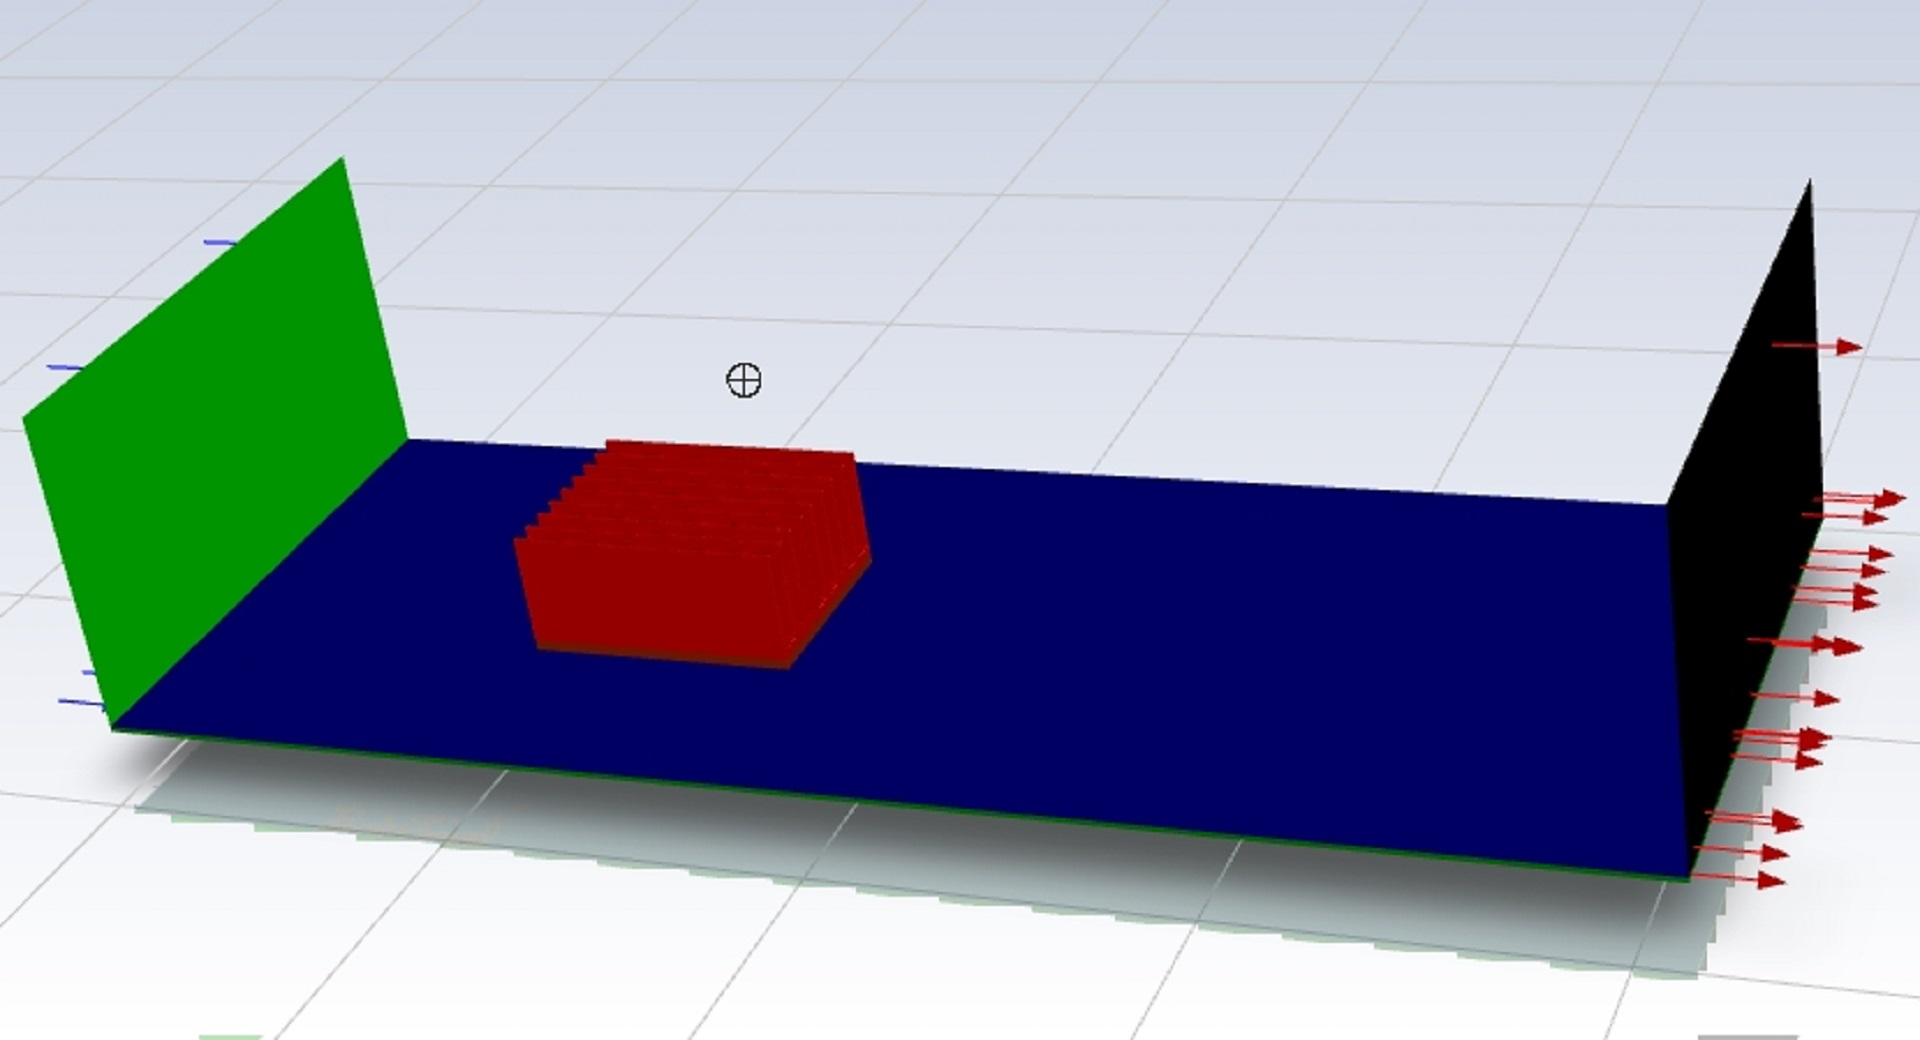
\includegraphics[width=\linewidth, trim={0 7cm 0 7cm}, clip]{title.jpg}}
\titlegraphic {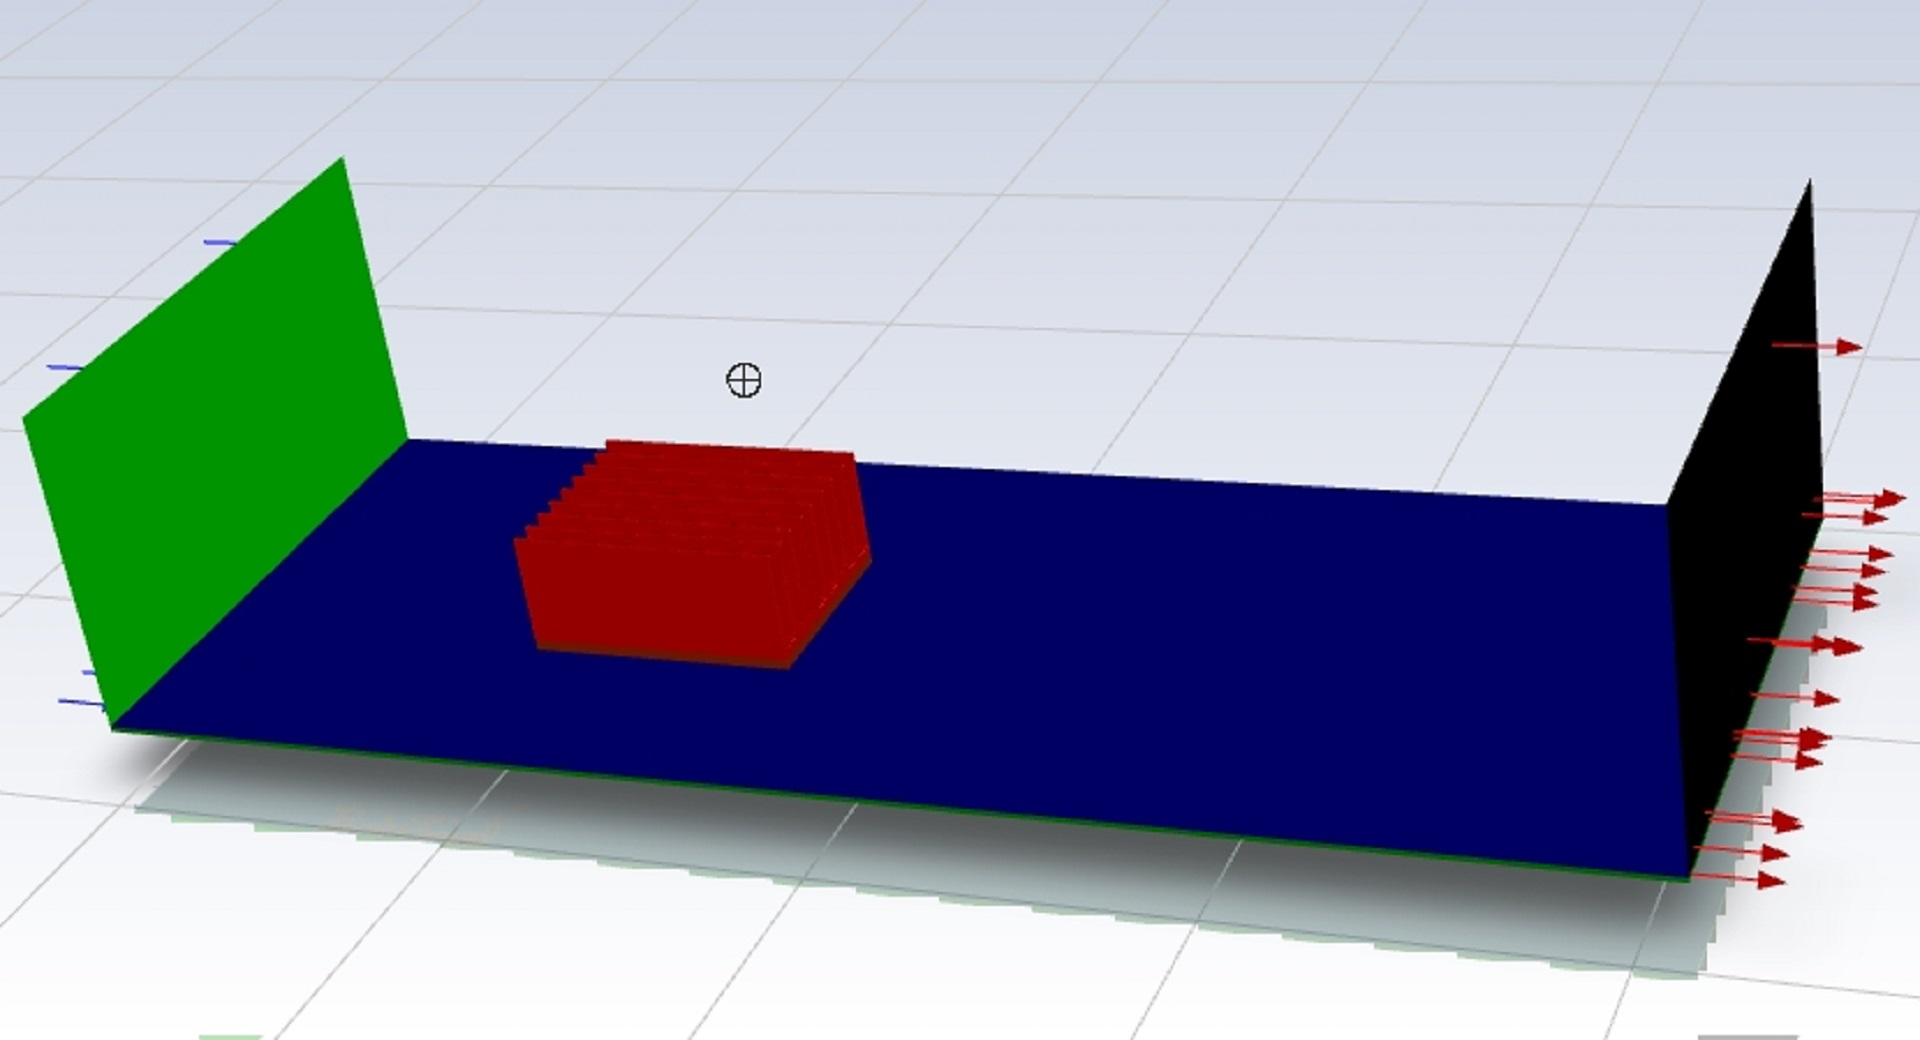
\includegraphics[width=\linewidth, trim={0 1cm 0 1cm}, clip]{title.jpg}}
% title graphic logo
\newcommand{\insertLogos}
{\centering 
\includegraphics[height=1.5cm]{hitlogo.jpg}\hspace{1em}
\includegraphics[height=1cm]{wenzi-logo.png}}
%
% Title page of presentation
%
\makeatletter
\setbeamertemplate{title page}
{
	\vbox{}
	%
	\begin{center}
		\begin{minipage}[c]{0.8\linewidth}
			 
			\inserttitlegraphic
			    
			\begin{beamercolorbox}[sep=8pt,center]{title}
				\usebeamerfont{title}
				\inserttitle%
			\end{beamercolorbox}
			%
			\vspace{-2ex}\
			\begin{beamercolorbox}[sep=8pt,center]{author}
				\usebeamerfont{author}\small\insertauthor
				\vspace{3ex}
			\end{beamercolorbox}
			%
			\begin{minipage}[c]{.5\textwidth}
				\insertLogos
			\end{minipage}
			%
			\begin{minipage}[c]{.5\textwidth}
				\small
				
				\vspace{0.5em}
				
				\Subject\\
				
				\vspace{0.5em}
				
				\PlaceAndTime\\
				
				\vspace{0.5em}
				
				\insertinstitute
			\end{minipage}%
			%
		\end{minipage}
	\end{center}
}
\makeatother
%
% start of document
%------------------------------------------------------------------------------
\begin{document}
%
% Title page
\begin{frame}[plain]
	\titlepage
\end{frame}
%
\begin{frame}{Agenda}
	\tableofcontents
\end{frame}
%
%
\section{Introduction}
\begin{frame}{Intro}
	%
	% \vfill
	This case demonstrates a simulation for the heat dissipation  problem of a electronic component  installed on the PCB, which is a typical conjugate heat transfer problem.
	\\
	\vfill

	\begin{figure}
		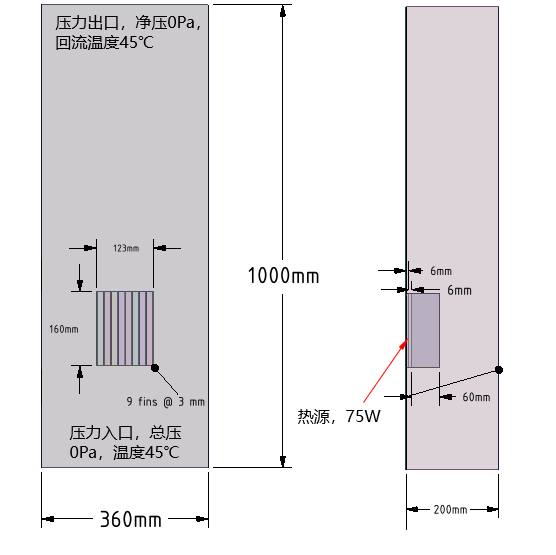
\includegraphics[height=7cm]{figure2.png}
		\caption{Problem description.}
	\end{figure}
	%

	\vfill
	%
\end{frame}
%
\begin{frame}{Geometry}
	Geometry model was built with SCDM. \textbf{Pay attention to share topology between parts.}
	\vfill
	\begin{figure}
		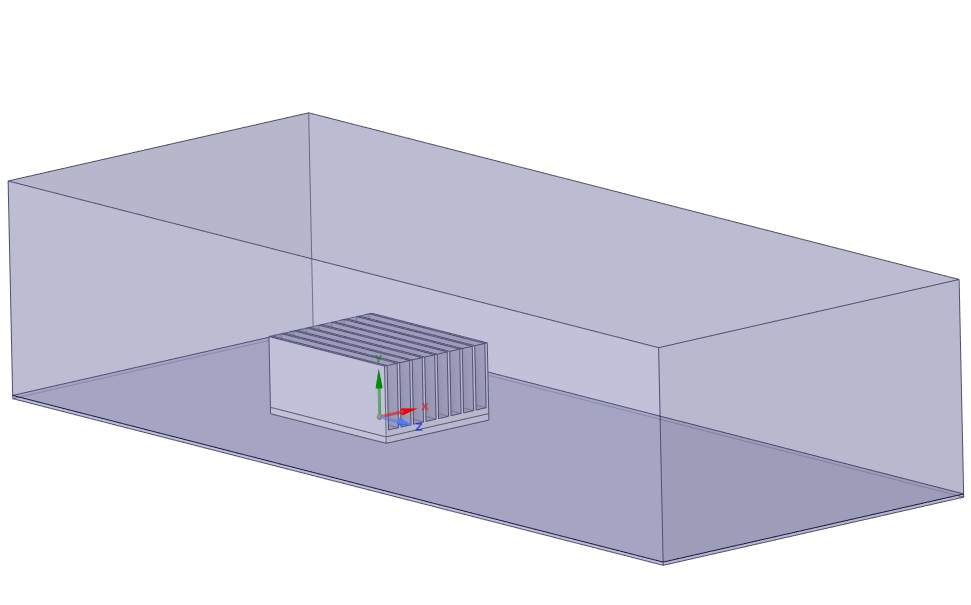
\includegraphics[width=8cm]{figure1.jpg}
		\caption{Geometry description.}
	\end{figure}	
\end{frame}
\section{CFD Simulation}
\begin{frame}{Meshing}
	
	\begin{figure}
		\includegraphics[width=8cm, trim={0 5cm 0 1cm}]{060622352924_1.pdf}
		\caption{Polyhedral unstructured mesh using FLUENT Meshing mode}
	\end{figure}	
\end{frame}
\begin{frame}{Model \& Methods}
	\begin{table}[]
		\begin{tabular}{l|l}
		\hline
		Model           & Settings           \\ \hline
		Heat   Transfer & Enabled            \\
		Radiation       & Surface to Surface \\
		Space           & 3D                 \\
		Time            & Steady             \\
		Viscous         & Laminar            \\ \hline
		\end{tabular}
		\caption[]{Model description.}
	\end{table}
\end{frame}
\begin{frame}{Model \& Methods}
	\begin{figure}
		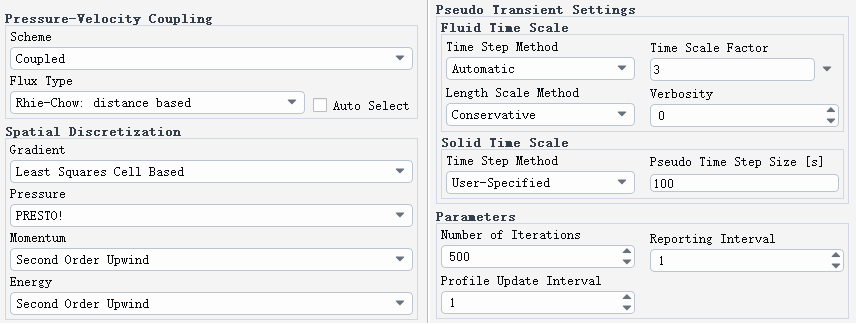
\includegraphics[width=10cm]{figure4.jpg}
		\caption{Method description.}
	\end{figure}	
\end{frame}

\begin{frame}{Materials}
	\begin{table}[]
		\begin{tabular}{|cc|}
		\hline
		\multicolumn{2}{|l|}{\textbf{air}}                                        \\ \hline
		\multicolumn{1}{|c|}{Density}              & incompressible ideal gas     \\ \hline
		\multicolumn{1}{|c|}{Cp (Specific Heat)}   & 1006.43 J/(kg K)             \\ \hline
		\multicolumn{1}{|c|}{Thermal Conductivity} & 0.0242 W/(m K)               \\ \hline
		\multicolumn{1}{|c|}{Viscosity}            & 1.7894e-05 kg/(m s)          \\ \hline
		\multicolumn{2}{|l|}{\textbf{component of heat source}}                   \\ \hline
		\multicolumn{1}{|c|}{Density}              & 1900 kg/m\textasciicircum{}3 \\ \hline
		\multicolumn{1}{|c|}{Cp (Specific Heat)}   & 795 J/(kg K)                 \\ \hline
		\multicolumn{1}{|c|}{Thermal Conductivity} & 10 W/(m K)                   \\ \hline
		\multicolumn{2}{|l|}{\textbf{component of PCB}}                           \\ \hline
		\multicolumn{1}{|c|}{Density}              & 1250 kg/m\textasciicircum{}3 \\ \hline
		\multicolumn{1}{|c|}{Cp (Specific Heat)}   & 1300 J/(kg K)                \\ \hline
		\multicolumn{1}{|c|}{Thermal Conductivity} & 0.35 W/(m K)                 \\ \hline
		\multicolumn{2}{|l|}{\textbf{component of heat sink}}                     \\ \hline
		\multicolumn{1}{|c|}{Density}              & 2719 kg/m\textasciicircum{}3 \\ \hline
		\multicolumn{1}{|c|}{Cp (Specific Heat)}   & 871 J/(kg K)                 \\ \hline
		\multicolumn{1}{|c|}{Thermal Conductivity} & 202.4 W/(m K)                \\ \hline
		\end{tabular}
		\caption[]{material properties}
		\end{table}
\end{frame}
\begin{frame}{Solution}
	\begin{figure}
		\includegraphics[width=10cm, trim={0 5cm 0 0cm}]{060622352924_3.pdf}
		\caption{Residuals.}
	\end{figure}	
\end{frame}
\begin{frame}{Solution}
	\begin{table}[]
		\begin{tabular}{|c|c|c|}
		\hline
		\multicolumn{1}{|l|}{}   & Simulation value   & Expected value \\ \hline
		Total heat transfer rate & 74.9808 W          & 75 W           \\ \hline
		Total mass flow rate     & 0.0000007916594 kg & 0              \\ \hline
		continuity residual      & 8.38303E-07        & 0              \\ \hline
		energy residual          & 2.08606E-07        & 0              \\ \hline
		x-velocity residual      & 0.000105974        & 0              \\ \hline
		y-velocity residual      & 0.000195162        & 0              \\ \hline
		z-velocity residual      & 0.000144551        & 0              \\ \hline
		\end{tabular}
		\caption{converge condition.}
		\end{table}	

\end{frame}
\section{Results}
\begin{frame}{Temperature}
	\begin{figure}
		\includegraphics[width=8cm, trim={0 4cm 0 1cm}]{060622352924_7.pdf}
		\caption{temperature distribution on the walls.}
	\end{figure}
\end{frame}
\begin{frame}{Temperature}
	\begin{figure}
		\includegraphics[width=8cm, trim={0 3cm 0 1cm}]{060622352924_5.pdf}
		\caption{temperature distribution on the heat sink.}
	\end{figure}	
\end{frame}
\begin{frame}{Temperature}
	\begin{figure}
		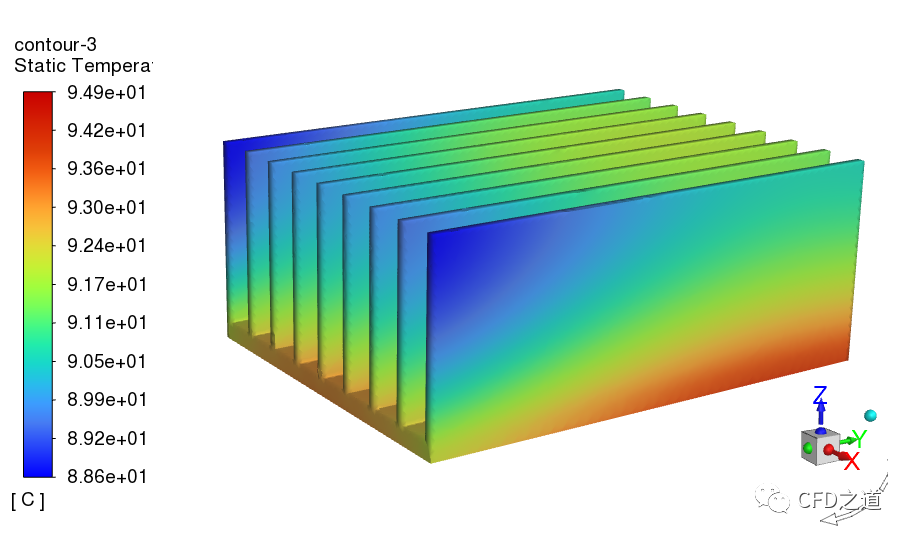
\includegraphics[width=8cm, trim={0 1cm 0 1cm}]{微信图片_20220606231543.png}
		\caption{temperature distribution on the heat sink in a similar case.}
	\end{figure}
\end{frame}
\begin{frame}{Temperature}
	\begin{figure}
		\includegraphics[width=8cm, trim={0 2cm 0 1cm}]{060622352924_6.pdf}
		\caption{temperature distribution on the bottom of heat sink.}
	\end{figure}
\end{frame}
\begin{frame}{Radiation Heat Flux}
	\begin{figure}
		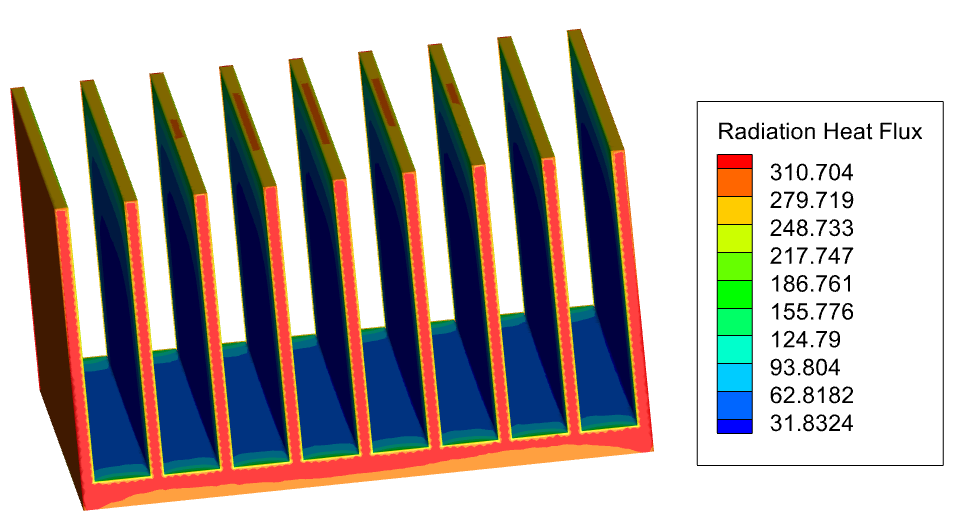
\includegraphics[width=8cm, trim={0 0cm 0 1cm}]{figure15.png}
		\caption{Radiation heat flux distribution on the heat sink.}
	\end{figure}
\end{frame}
\begin{frame}{Temperature}
	\begin{figure}
		\includegraphics[width=8cm, trim={0 4cm 0 1cm}]{060622352924_8.pdf}
		\caption{Temperature distribution on the center plane of fins.}
	\end{figure}
\end{frame}
\begin{frame}{Velocity}
	\begin{figure}
		\includegraphics[width=8cm, trim={0 5cm 0 1cm}]{060622352924_10.pdf}
		\caption{Contour of Velocity on the center plane of fins.}
	\end{figure}	
\end{frame}
\begin{frame}{Velocity}
	\begin{figure}
		\includegraphics[width=8cm, trim={0 5cm 0 1cm}]{060622352924_9.pdf}
		\caption{Streamline of Velocity on the center plane of fins.}
	\end{figure}	
\end{frame}
\begin{frame}{No-radiation case}
	% \vfill
	\begin{figure}[htbp]
		\centering
		\subfigure[]
		{
		%  \begin{minipage}{5cm}
		  \centering
		  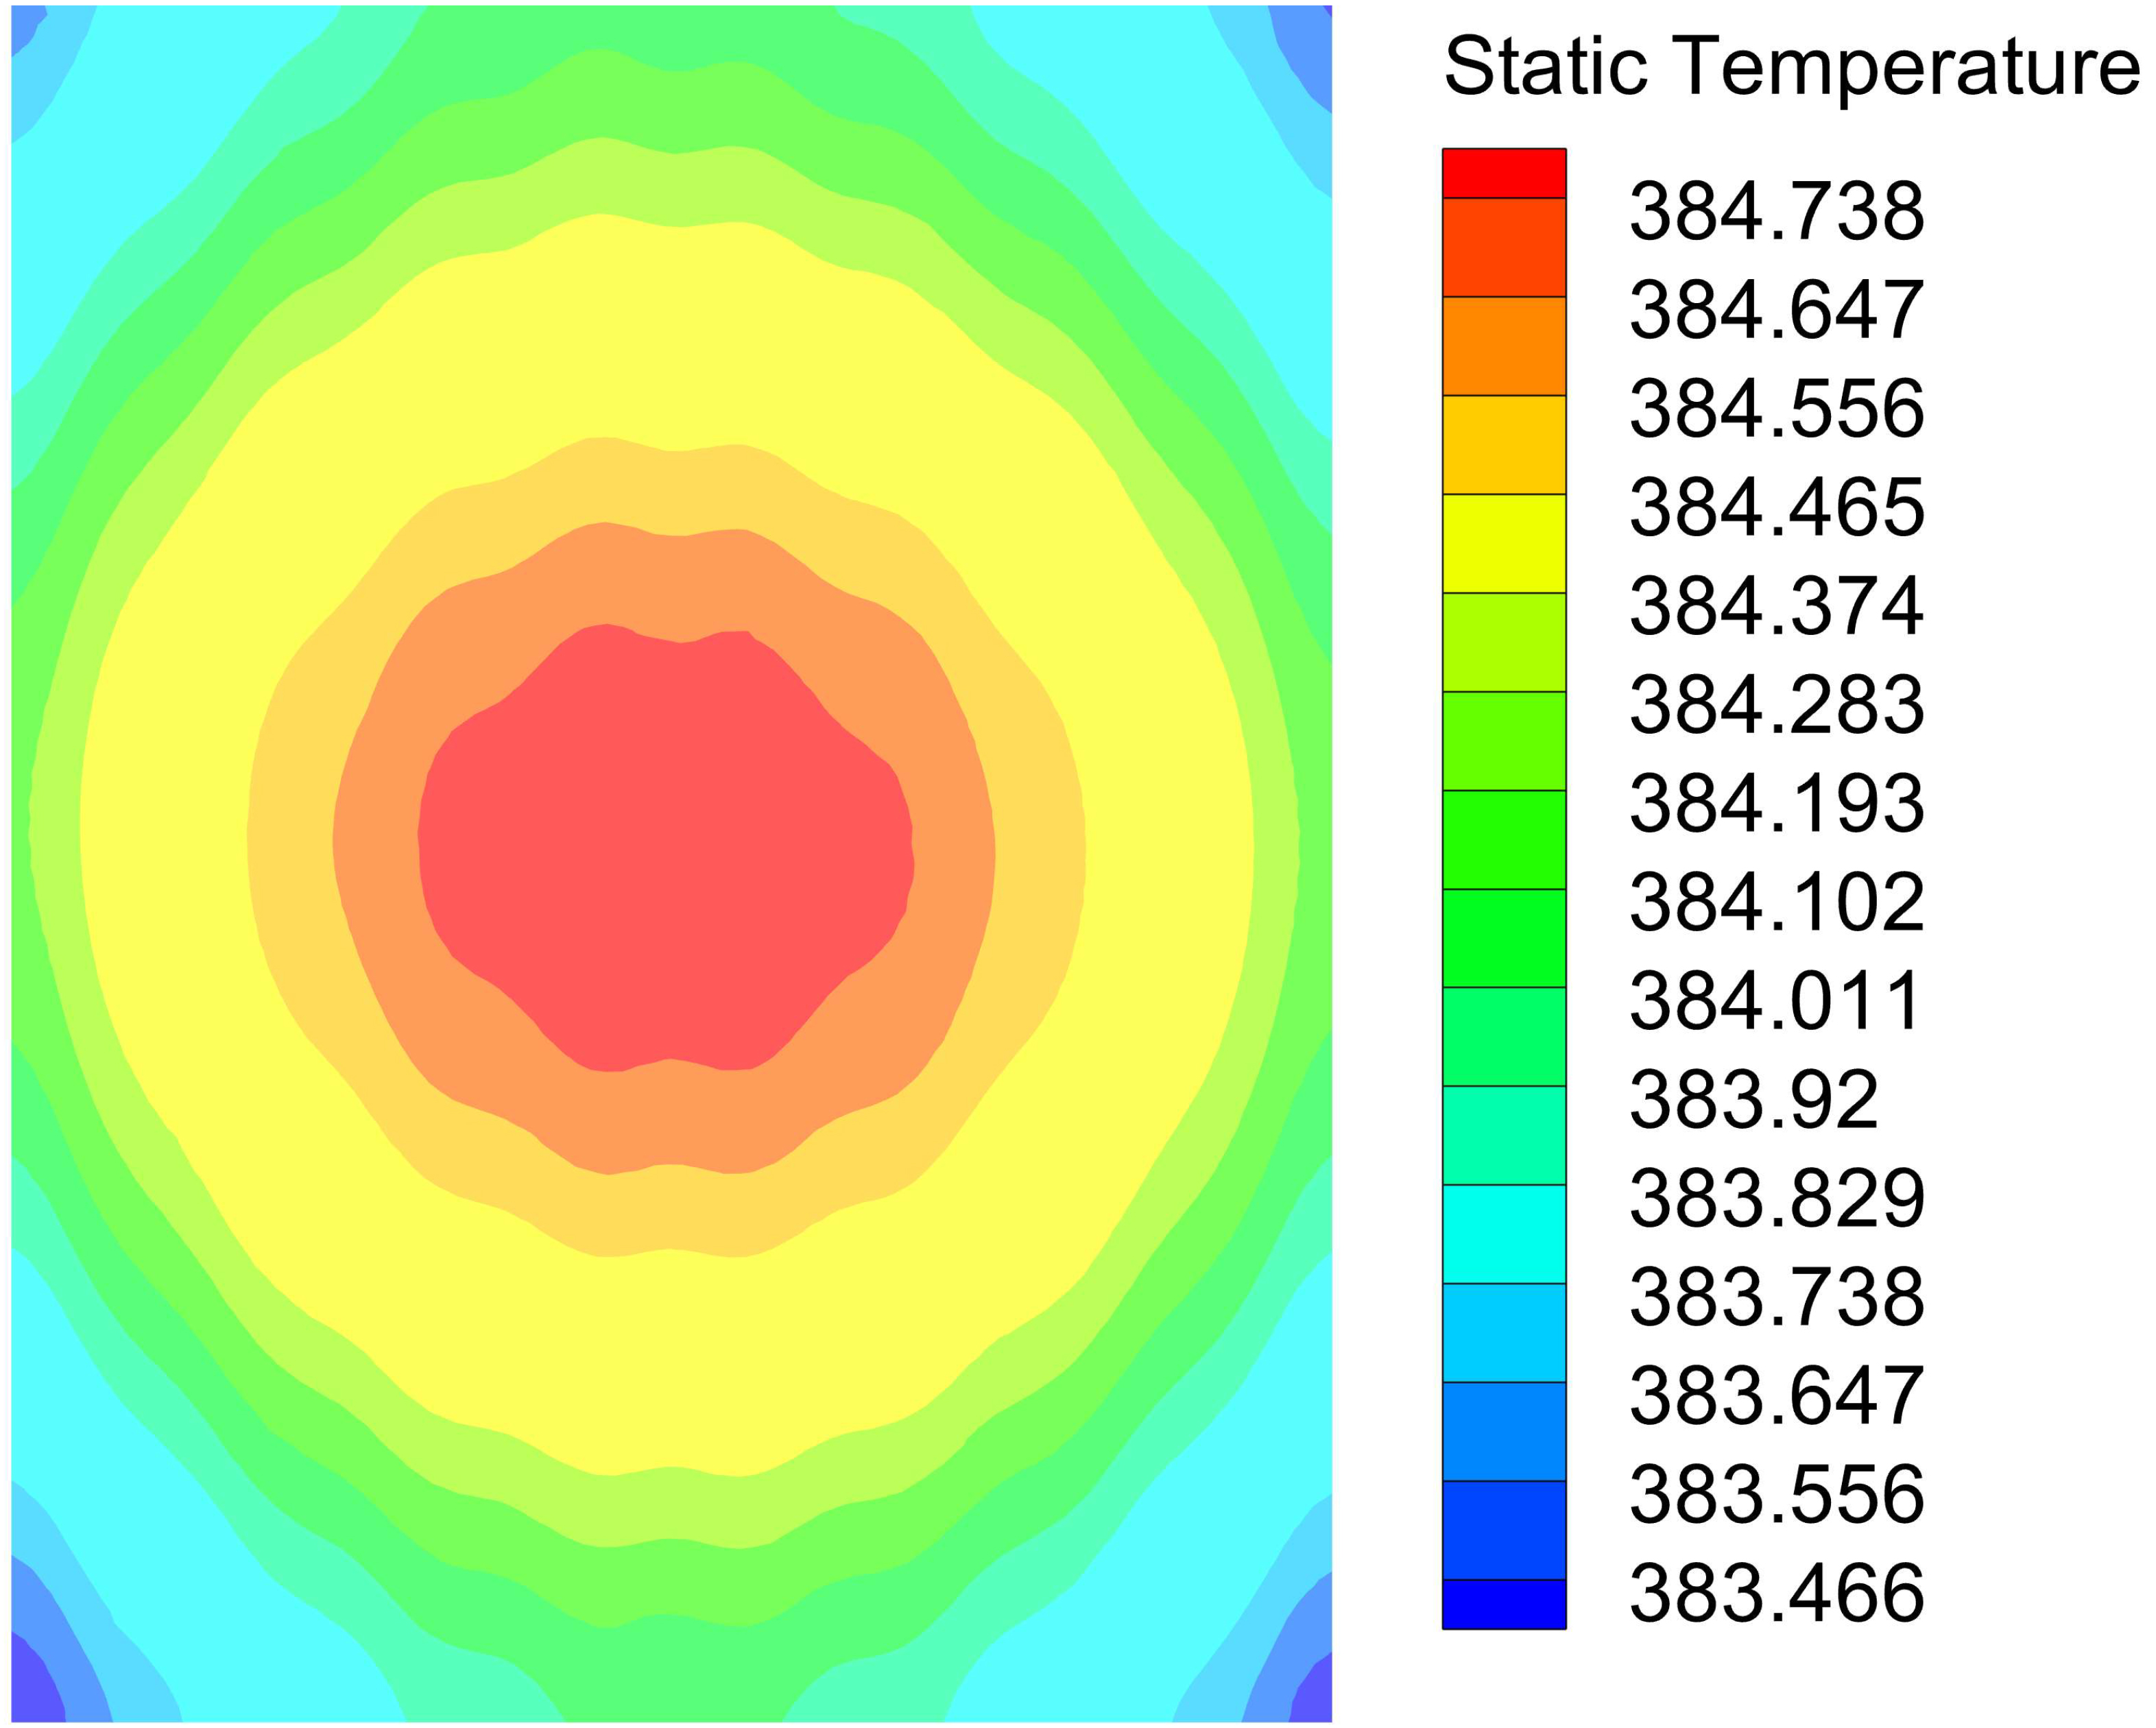
\includegraphics[scale=0.7,width=5cm]{figure14-no.jpg}
		%  \end{minipage}
		}
		   \subfigure[]
		   {
			% \begin{minipage}{5cm}
			 \centering
			 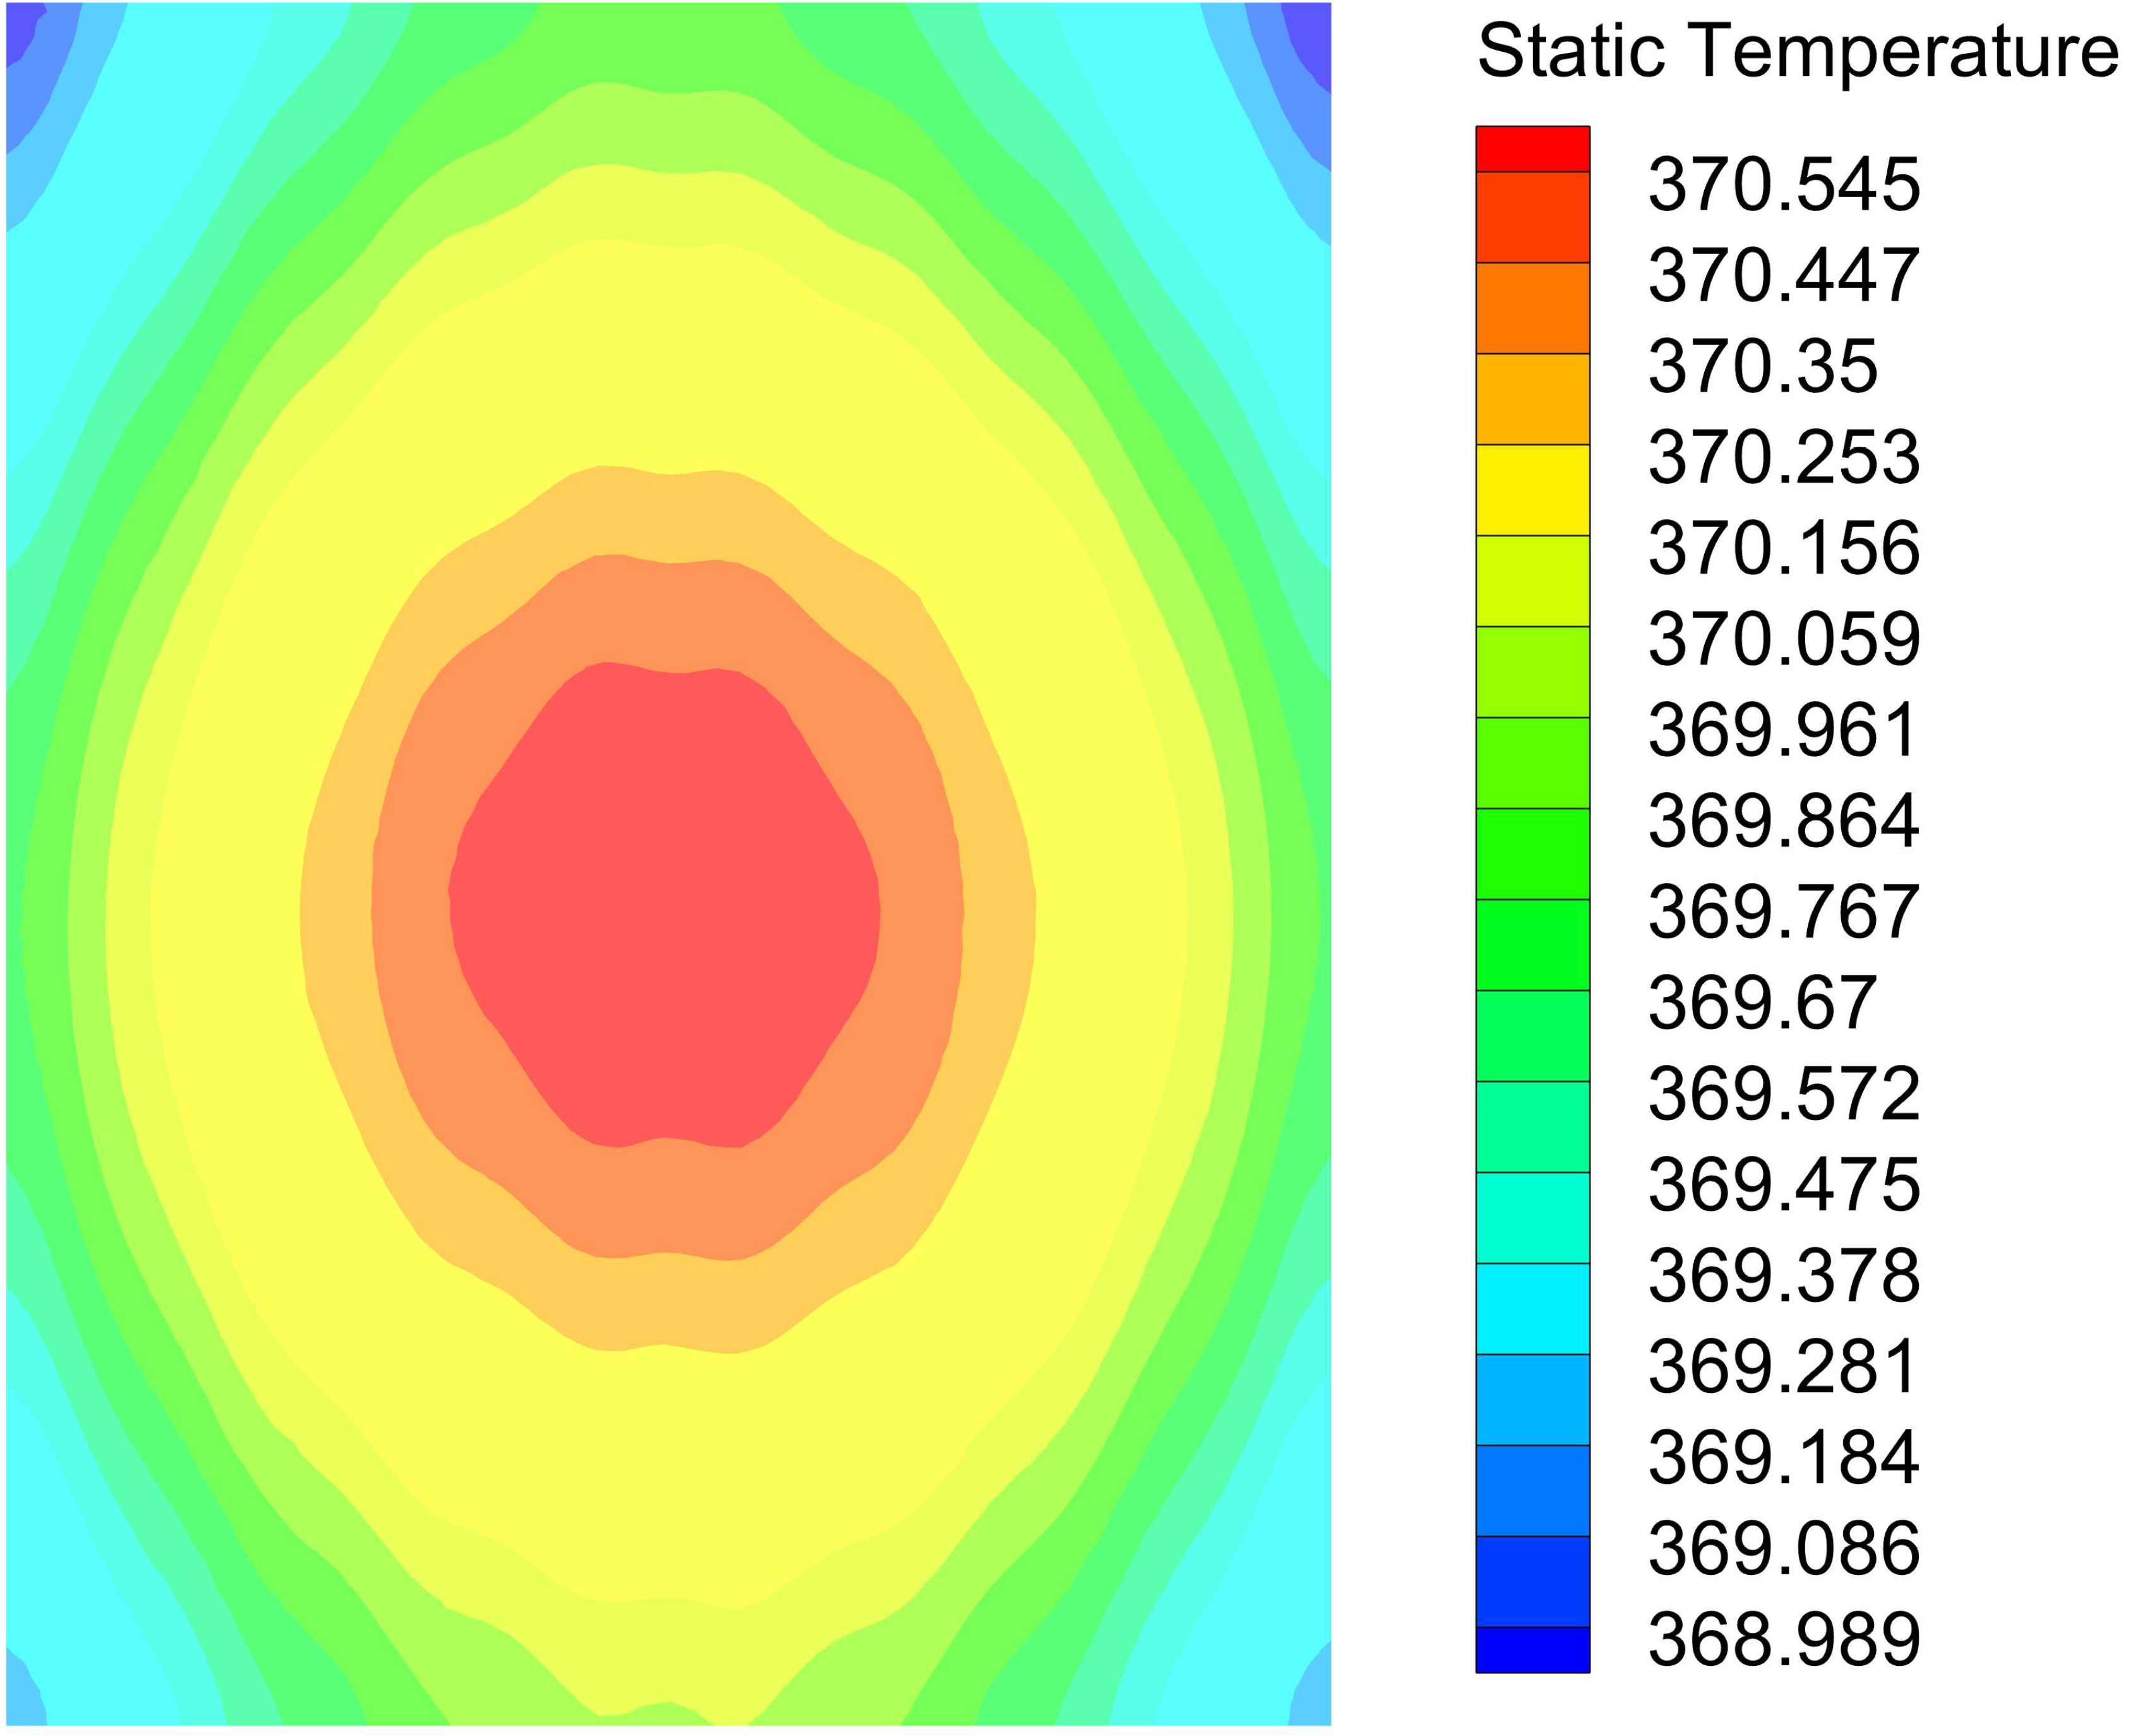
\includegraphics[scale=0.7,width=5cm]{figure14-0.jpg}
			% \end{minipage}
		   }
	   \caption{Temperature of the heat source surface before(a) and after(b) applying S2S model.}
	   \label{fig:14}
	   \end{figure}
\end{frame}
% \section{Topic}
% %
% \begin{frame}{Topic Slide 1}
% 	%
% 	\begin{columns}[totalwidth=\linewidth]
% 		\begin{column}{0.5\columnwidth}
% 			%
% 			Here's some text with a citation \cite{Book4}. Heres another one \cite{Book5}. Take a look at figure \ref{fig:Example} and table \ref{tab:Example}.
% 			\vspace{2ex}
% 			%
% 			\begin{table}[c]
% 				\centering
% 				\begin{tabular}{c|c|c}
% 					Object & Length & Height \\ \hline
% 					A      & 2.52   & 3.53   \\ \hline
% 					B      & 1.90   & 5.30   \\ \hline
% 				\end{tabular}
% 				\caption{Exemplary table.}
% 				\label{tab:Example}
% 			\end{table}
% 			%
% 		\end{column}
% 		\begin{column}{0.5\columnwidth}
% 			\begin{figure}
% 				\centering
% 				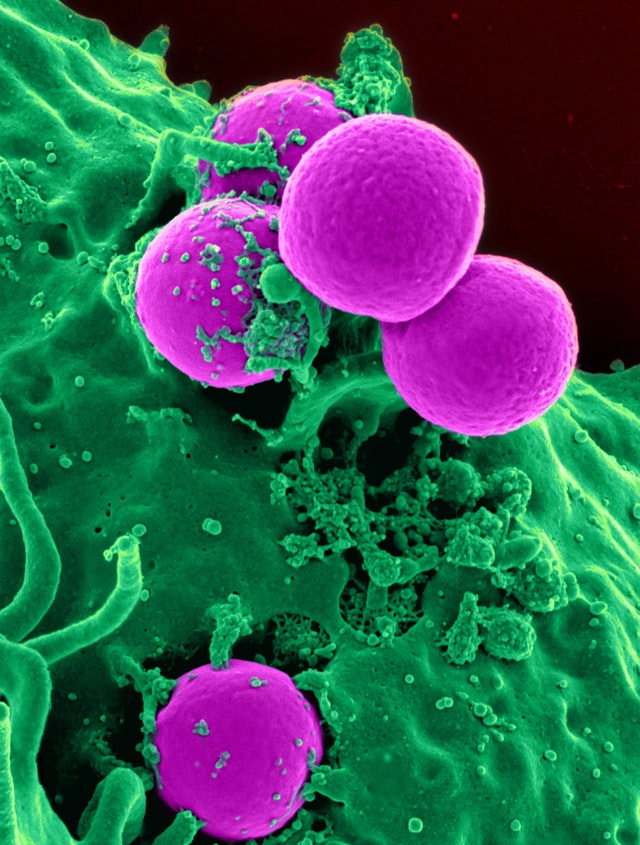
\includegraphics[height=0.5\paperheight]{pexels-pixabay-45239.jpg}
% 				\caption{Exemplary image. Source: \cite{PixMicroscope}}
% 				\label{fig:Example}
% 			\end{figure}
% 		\end{column}
% 	\end{columns}
% 	%
% \end{frame}
% %
% \begin{frame}{Topic Slide 2}
% 	%
% 	\begin{block}{Observation}
% 		This is an Observation Block.
% 	\end{block}
% 	%
% 	\begin{exampleblock}{Example}
% 		This is an Example Block.
% 	\end{exampleblock}
% 	%
% 	\begin{alertblock}{Alert}
% 		This is an Alert Block.
% 	\end{alertblock}
% 	%
% 	\vfill
% 	This leads to the following equation:
% 	\begin{equation}
% 		M = \frac{2\pi}{x^5 - y^3 + \sin(x)} \cdot \int_{a}^{b} f(x)^2 \,dx
% 	\end{equation}
% \end{frame}
% %
% %
% \section{Outlook}
% \begin{frame}{Outlook}
% 	%
% 	\textbf{List}\\
% 	\begin{itemize}
% 		\item Pri sonet labore expetenda
% 		      \begin{itemize}
% 		      	\item Svix te wisi atqui inermis
% 		      	\item  Cum dolor delenit argumentum et
% 		      \end{itemize}
% 		\item no vim quidam probatus senserit
% 		\item accommodare necessitatibus ad quo
% 		\item integre persecuti efficiantur at pro
% 	\end{itemize}
% 	%
% 	\vfill
% 	%
% 	\textbf{List 2}\\
% 	\begin{enumerate}
% 		\item no vis patrioque reprehendunt
% 		\item partem definitiones nam
% 		\item vel wisi dignissim voluptatibus ut
% 	\end{enumerate}
% 	%
% \end{frame}
% %
% %------------------------------------------------------------------------------
% %
% \section{Sources}
%
% \begin{frame}{Sources (1)}
% 	\textbf{Image Sources}\\[2ex]
% 	\small Title page:
% 	\fullcite{PixBoard}
% 	\vspace{2ex}

% 	\printbibliography[keyword=pic]
% \end{frame}
% %
% \begin{frame}
% 	\frametitle{Sources (2)}
% 	\textbf{Sources}\\
% 	\printbibliography[keyword=inf]
% 	\vfill
% 	%
% 	\textbf{Additional Literature}
% 	\small
% 	\begin{itemize}
% 		\item \fullcite{Book1}
% 		\item \fullcite{Book2}
% 		\item \fullcite{Book3}
% 	\end{itemize}
% \end{frame}
% %
\begin{frame}{}
	\usebeamerfont{AAA}
	\begin{center}
		\Huge Thanks for attention!\\[2ex]
		% \small Please feel free to ask any questions
		% \vspace{10ex}

		% Contact:\\
		% \Contactmail
	\end{center}
\end{frame}
%
%------------------------------------------------------------------------------
\end{document}
